% 1986 年全国卷理科第 8 题：正方形折叠示意图
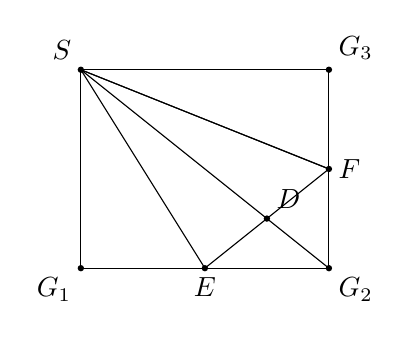
\begin{tikzpicture}[scale=1.05,>=stealth]
  \coordinate (S) at (0,2.4);
  \coordinate (G3) at (3,2.4);
  \coordinate (G2) at (3,0);
  \coordinate (G1) at (0,0);
  \coordinate (E) at (1.5,0);
  \coordinate (F) at (3,1.2);
  \coordinate (D) at (2.25,0.6);
  \draw (S)--(G3)--(G2)--(G1)--cycle;
  \draw (S)--(E)--(F)--cycle;
  \draw (S)--(F);
  \draw (S)--(G2);
  \draw (E)--(G2);
  \draw (F)--(G3);
  \fill (S) circle (1.1pt) node[above left] {$S$};
  \fill (G3) circle (1.1pt) node[above right] {$G_3$};
  \fill (G2) circle (1.1pt) node[below right] {$G_2$};
  \fill (G1) circle (1.1pt) node[below left] {$G_1$};
  \fill (E) circle (1.1pt) node[below] {$E$};
  \fill (F) circle (1.1pt) node[right] {$F$};
  \fill (D) circle (1.1pt) node[above right] {$D$};
\end{tikzpicture}
